\documentclass[8pt]{beamer}

% Import packages
\usepackage{siunitx}
\usepackage{graphicx}
\usepackage{calc}
\usepackage{textpos}
\usepackage{physics}
\usepackage{tabularx}
\usepackage{amsmath}
\usepackage{tikz}
\usepackage{xparse}% So that we can have two optional parameters
\usepackage{mathtools}
\usepackage{eso-pic}
\usepackage{mdframed}
\usepackage{newunicodechar}
\usepackage{chemformula}
\usepackage{subfig}
\usepackage[justification=justified]{caption}
\usepackage{todonotes}
\usepackage{listings}
\usepackage{subfig} 
\usepackage{tcolorbox}
\usepackage[qm]{qcircuit}

% LISTING SETTINGS
\definecolor{codegray}{rgb}{0.5,0.5,0.5}
\definecolor{commentcolour}{rgb}{0.43,0.63,0.65}
\definecolor{darkgreen}{rgb}{0.0, 0.5, 0.0}
\lstdefinestyle{myPython}{
    language=Python,
    backgroundcolor=\color{white},
    commentstyle=\color{commentcolour},
    keywordstyle=\bfseries\color{darkgreen},
    numberstyle=\tiny\color{codegray},
    stringstyle=\color{hot},
    basicstyle=\ttfamily\footnotesize,
    breakatwhitespace=false,
    breaklines=true,
    captionpos=b,
    keepspaces=true,
    arc=5mm,
    showspaces=false,
    showstringspaces=false,
    showtabs=false,
    tabsize=2
}

% Define my colors
\colorlet{myred}{red!65!black}
\definecolor{myblue}{RGB}{229,230,238}
\colorlet{mydarkblue}{blue!35!black}
\definecolor{linkcolor}{rgb}{0,0,0.65} %hyperlink
\definecolor{linescolor}{rgb}{0.65,0.16,0.16}

% Select theme
\usetheme{Madrid}
% Change theme color from blue to red
\colorlet{beamer@blendedblue}{myred}

% Select font
\setbeamerfont{title}{size=\huge,series=\bfseries,parent=structure,family=\fontfamily{\sfdefault}\selectfont}
\setbeamerfont{subtitle}{size=\Large,series=\bfseries,parent=structure, family=\fontfamily{\sfdefault}\selectfont}
\setbeamerfont{frametitle}{size=\LARGE,   family=\fontfamily{\sfdefault}\selectfont,series=\bfseries}
\setbeamerfont{framesubtitle}{size=\large,family=\fontfamily{\sfdefault}\selectfont,series=\normalfont}
\setbeamerfont{author}{size=\large,series=\bfseries,parent=structure,family=\fontfamily{\sfdefault}\selectfont}
\setbeamerfont{date}{size=\normalsize,series=\bfseries,parent=structure,family=\fontfamily{\sfdefault}\selectfont}
\setbeamerfont{institute}{size=\normalsize,series=\bfseries,parent=structure,family=\fontfamily{\sfdefault}\selectfont}

% Remove navigation bar
\beamertemplatenavigationsymbolsempty

%%% theme blocks style
\useinnertheme{rectangles}
\setbeamertemplate{blocks}[default]
\setbeamertemplate{title page}[default][rounded=true]

% To set titlepage
\defbeamertemplate*{footline}{noslidenum theme}
{
  \leavevmode%
  \hbox{%
    \begin{beamercolorbox}[wd=0.3\paperwidth,ht=2.25ex,dp=1ex,center]{author in head/foot}%
      \usebeamerfont{author in head/foot}\textbf{\insertshortauthor}
    \end{beamercolorbox}%
    \hspace{0.05pt}%
    \begin{beamercolorbox}[wd=0.4\paperwidth,ht=2.25ex,dp=1ex,center]{title in head/foot}%
      \usebeamerfont{title in head/foot}{
   \hypersetup{linkcolor=white}\textbf{\insertshorttitle}}
    \end{beamercolorbox}%
    \hspace{0.05pt}%
    \begin{beamercolorbox}[wd=0.25\paperwidth,ht=2.25ex,dp=1ex,center]{date in head/foot}%
      \usebeamerfont{date in head/foot}\textbf{\insertshortdate}
    \end{beamercolorbox}%
    \hspace{-0.2pt}%
    \begin{beamercolorbox}[wd=0.05\paperwidth,ht=2.25ex,dp=1ex,center]{date in head/foot}
      {\fontfamily{\sfdefault}\selectfont\color{white}\textbf{\insertframenumber}/\textbf{\inserttotalframenumber}}
    \end{beamercolorbox}
  }%
  \vskip0pt%
}

% Set image in titlepage
\addtobeamertemplate{frametitle}{}{%
	\begin{textblock*}{100mm}(.85\textwidth,-1.1cm) %before -0.9cm
		
\includegraphics[height=0.85cm]{images/logo/unipd_logo_white.png}
	\end{textblock*}
}

% Set title
\title[Two-qubit CZ gate with trapped neutral atoms]{
	
\includegraphics[height=2cm]{images/logo/unipd_logo_white.png}\\
	~\\
	\textbf{ \Large
		Two-qubit CZ gate implementation with trapped neutral atoms: \\ a numerical simulation
	}
}

% Set institute
\institute{Quantum Information and Computing \\ (a.y. 2020/21) }

% Set author
\author[Alice Pagano - Michele Puppin]{\small%
    \parbox{2.5cm}{Alice Pagano}\parbox{2.5cm}{Mat. 1236916} \parbox{3.8cm}{\bf\href{mailto:alice.pagano@studenti.unipd.it}{\texttt{\color{linkcolor}alice.pagano@studenti.unipd.it}}} 
    \\ \vspace{0.1cm}
    \parbox{2.5cm}{Michele Puppin}\parbox{2.5cm}{Mat. 1227474} \parbox{3.8cm}{\bf\href{mailto:michele.puppin@studenti.unipd.it}{\texttt{\color{linkcolor}michele.puppin@studenti.unipd.it}}}}

% Set date
\date{22 March 2021}




\begin{document}

\begin{frame}[plain]
    \titlepage
\end{frame} 

\setcounter{framenumber}{0}

\begin{frame}[c]{Chain of N-qubits}
\framesubtitle{Numerical simulation}
\begin{itemize}
    \item Numerical simulation of a \textbf{chain of $N$-qubit}
    \item The \textbf{CZ gate} is applied between consequent qubits, assuming \textbf{perfect blockade regime}
    \item One-dimensional array of atoms $\rightarrow$ each time the \textbf{two-qubit CZ gate} acts on a \textbf{pair of atoms}, the interaction with the other atoms is neglected
\end{itemize}

\begin{equation*}
\Qcircuit @C=0.8em @R=1.1em {
\lstick{\ket{1}_0}	& \ctrl{1}	& \qw      & \qw & \qw &\qw & \qw            & \qw & \qw & \qw & \qw & \qw & \qw\\
\lstick{\ket{0}_1}	& \gate{Z}	& \ctrl{1} & \qw & \qw &\qw & \qw            & \qw & \qw & \qw & \qw & \qw & \qw\\
\lstick{\dots}	    & \qw 	    & \gate{Z} & \qw & \qw &\qw & \qw            & \qw & \qw & \qw & \qw & \qw & \qw\\
                    &           & \vdots   &     &  \vdots   &    &    & \vdots     &     &     &     &     &    \\
\lstick{\dots}      & \qw	    & \qw      & \qw & \qw &\qw & \qw       & \qw & \qw & \qw & \ctrl{1} & \qw & \qw\\
\lstick{\ket{1}_N}	& \qw	    & \qw      & \qw & \qw &\qw & \qw       & \qw & \qw & \qw & \gate{Z}& \qw & \qw\\
}
\end{equation*}

\end{frame}

\begin{frame}[c]{Chain of N-qubits}
\framesubtitle{Implementation}

\begin{itemize}
    \item Obtain the \textbf{behavior} of the map in Eq. between the \textbf{first} and \textbf{last qubits}
      \begin{equation*}
    \begin{aligned}
        \ket{00} & \rightarrow \ket{00} \\
        \ket{01} & \rightarrow \ket{01} e^{i\phi} \\
        \ket{10} & \rightarrow \ket{10} e^{i\phi}\\
        \ket{11} & \rightarrow \ket{11} e^{i(2\phi-\pi)}\\
    \end{aligned}
    \label{eq:CZ-gate-map}
\end{equation*}
    \item \textbf{First} and \textbf{last qubits} can be \textbf{initialized} either in state $\ket{0}$ or $\ket{1}$
    \item All the other qubits in the chain are \textbf{initialized} in $\ket{0}$
    \item The state vector of the \textbf{$N$-qubit} system is the \textbf{tensor product} of the \textbf{subsystems} as:
    \begin{equation*}
        \ket{\psi} = \ket{q_1} \otimes \dots \otimes \ket{q_N}
    \end{equation*}
    \item Starting from the first qubit, we \textbf{apply} the two-qubit CZ gate \textbf{iteratively}. 
    \item In the $i$-th iteration, the total \textbf{Hamiltonian} of the chain $H_{chain}$ is:
    \begin{equation*}
    H_{chain,i}^{(N)} =  \underbrace{\mathbb{I}_3  \otimes \dots \otimes \mathbb{I}_3}_{i-1} \otimes H_{\text{CZ}} \otimes \underbrace{ \mathbb{I}_3  \otimes \dots \otimes \mathbb{I}_3}_{N-i-1}.
    \end{equation*}
    \item Hamiltonian of \textbf{dimension} $3^N\times 3^N$
\end{itemize}   
\end{frame}

\begin{frame}[c]{Time-dependent Schr{\"o}dinger equation solvers
}
\framesubtitle{Numerical methods}

\begin{itemize}
    \item As \textbf{longer chains} are considered, the dimension of the total Hamiltonian of the system \textbf{scales} as $3^N \times 3^N$
    \item Given the Hamiltonian $H$ of the system, the \textbf{time-dependent Schrödinger equation} can be solved as:
    \begin{equation*}
        \ket{\psi(t)} = U(t) \ket{\psi(0)}, \qquad U(t)=e^{-iHt/\hbar}
    \end{equation*}
    \item The \textbf{time evolution} of the system can become \textbf{computationally challenging} for large $N$.
    \item We consider several time-dependent Schr{\"o}dinger \textbf{equation solvers}, along with some optimizations, in order to test their performances
    \item We implement these algorithms using \textbf{different coding environment} and \textbf{libraries implementation} both on CPU and GPU
\end{itemize}

\end{frame}

\begin{frame}[c]{Time-dependent Schr{\"o}dinger equation solvers
}
\framesubtitle{Implementations}

\textbf{NumPy implementation}
\begin{itemize}
    \item Support for large, multi-dimensional arrays
    \item Collection of high-level mathematical functions
    \item Coded in well-optimized C code
    \item SciPy provides sparse array libraries
    \item Plays well with parallel computing
\end{itemize}
\vspace{0.5cm}
\textbf{TensorFlow implementation}
\begin{itemize}
    \item Optimized to deal with large matrices
    \item Can be easily executed on GPU thanks to CUDA
\end{itemize}
\vspace{0.5cm}
\textbf{Fortran implementation}
\begin{itemize}
    \item One of the most powerful language for scientific computation with LAPACK routines for linear algebra
    \item Its design allows the compiler to perform stronger optimizations
\end{itemize}

\end{frame}

\begin{frame}[c]{Time-dependent Schr{\"o}dinger equation solvers
}
\framesubtitle{Spectral method}
\begin{itemize}
    \item We compute the \textbf{unitary time evolution} of the system as \begin{equation*}
    \ket{\psi(t)} = U(t) \ket{\psi(0)}, \qquad U(t)=e^{-iHt/\hbar}
    \end{equation*}
    \item The system Hamiltonian can be diagonalized $H = PDP^{-1}$, where $D$ is the diagonal matrix and $P$ is the eigenvectors matrix.
    \item The exponential matrix can be computed as: 
    \begin{equation*}
    e^{-iHt} = P e^{-iDt} P^{-1}
    \end{equation*}
    \vspace{0.5cm}
    \item \textbf{NumPy} $\rightarrow$ matrix diagonalization with {\bfseries\texttt{numpy.linalg.eigh}}, matrix inversion with {\bfseries\texttt{numpy.linalg.inv}}
    \item \textbf{TensorFlow} $\rightarrow$ matrix exponential with {\bfseries\texttt{tensorflow.linalg.expm}}
    \item \textbf{Fortran} $\rightarrow$ matrix diagonalization with {\bfseries\texttt{\_heev}}, matrix inversion with  {\bfseries\texttt{\_getrf}} and {\bfseries\texttt{\_getri}} LAPACK routines
\end{itemize}
\end{frame}

\begin{frame}[c]{Time-dependent Schr{\"o}dinger equation solvers
}
\framesubtitle{Crank-Nicolson method}
\begin{itemize}
    \item Given a discrete time step $\Delta t$, solving time-dependent Schr{\"o}dinger equation is equivalent to solve the linear system:
    \begin{equation*}
    \qty( 1 + \frac{iH\Delta t}{2} )    \psi(x,t+\Delta t) = \qty( 1 - \frac{iH\Delta t}{2} ) \psi(x,t).
    \end{equation*}
    \item By iterating the procedure $n_{iter}$ times, we obtain the time evolution for time $T = \Delta t \times n_{iter}$
    \vspace{0.5cm}
    \item \textbf{NumPy} $\rightarrow$ linear system solved with  {\bfseries\texttt{numpy.linalg.solve}}
    \item \textbf{TensorFlow} $\rightarrow$ analogous resolution using {\bfseries\texttt{tensorflow.linalg}} module
\end{itemize}

\end{frame}


\begin{frame}[c]{Time-dependent Schr{\"o}dinger equation solvers
}
\framesubtitle{Crank-Nicolson method with LU decomposition}

\begin{itemize}
    \item An invertible matrix $A$ can be decomposed into two factors $LU$, where $L$ is a lower and a $U$ an upper triangular matrix.
    \item The linear system $A\boldsymbol{x} = \boldsymbol{y}$ can be recasted as: 
    \begin{equation*}
    \begin{cases}
        L\boldsymbol{z} = \boldsymbol{y} \\
        U\boldsymbol{x} = \boldsymbol{z} \\
    \end{cases}
    \end{equation*}
    \item In our case the matrix $A$ is fixed and the system has to be solved many times for different $\boldsymbol{x}$ and $\boldsymbol{y}$
    \vspace{0.5cm}
    \item \textbf{NumPy} $\rightarrow$ compute the LU decomposition with {\bfseries\texttt{scipy.linalg.lu}} function and solve the systems with the {\bfseries\texttt{scipy.linalg.solve\_triangular}} function
    \item \textbf{TensorFlow} $\rightarrow$ analogous resolution using {\bfseries\texttt{tensorflow.linalg}} module
    \vspace{0.5cm}
    \item The total Hamiltonian of the $N$-qubits system is a \textit{sparse matrix}
    \item \textbf{NumPy} $\rightarrow$ matrices are transformed into \texttt{csc\_matrix}
    \item optimized functions are used for LU decomposition and triangular systems solving
\end{itemize}
\end{frame}

\begin{frame}[c]{Noise effects}
\framesubtitle{Gaussian noise on $\Omega \tau$ and  $\Delta/\Omega$}
\begin{figure}[H]
\begin{minipage}[c]{0.49\linewidth}
\subfloat[][$\Omega \tau$]{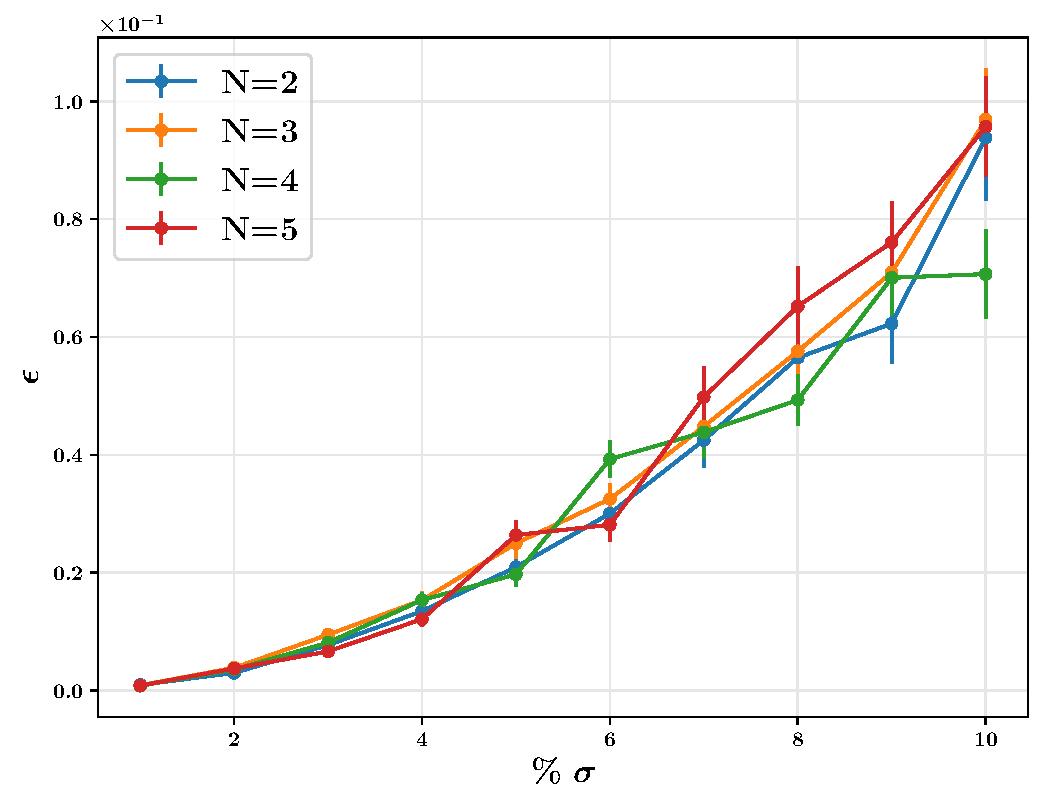
\includegraphics[width=1.0\textwidth]{images/two-qubit-system/chain/chain_sigma_tau.pdf} \label{fig:chain_tau} }
\end{minipage}
\begin{minipage}[]{0.49\linewidth}
\centering
\subfloat[][$\Delta/\Omega$]{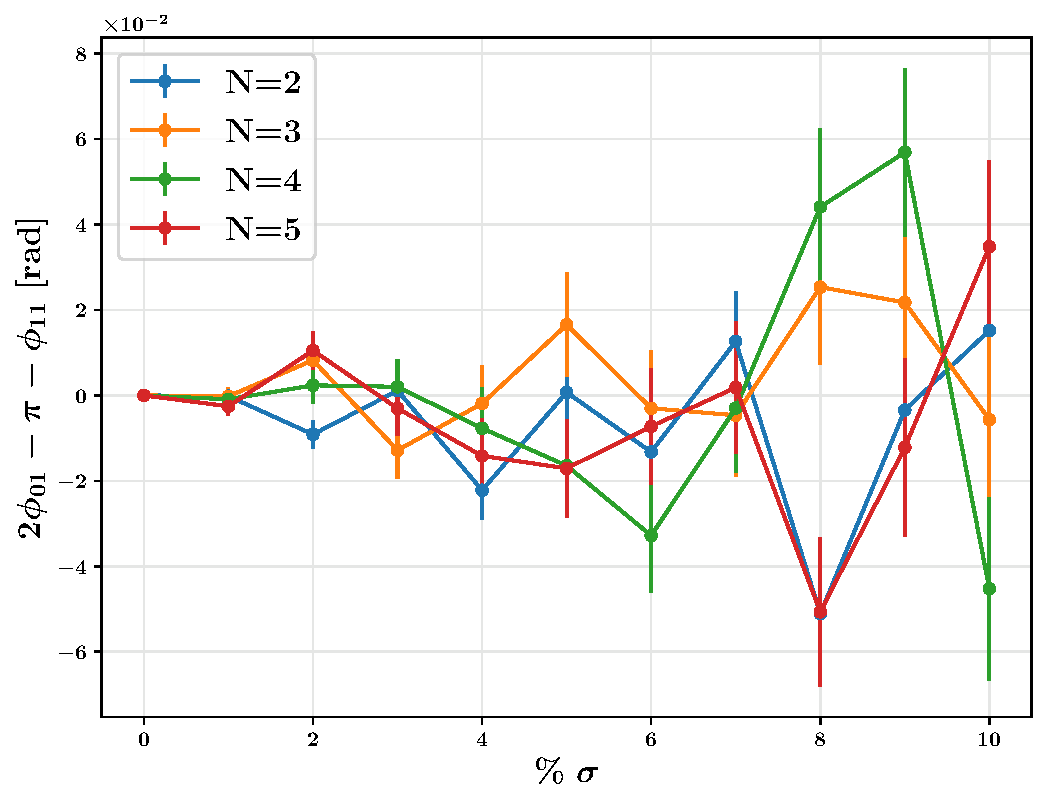
\includegraphics[width=1.0\textwidth]{images/two-qubit-system/chain/chain_phase_sigma_delta.pdf}  \label{fig:chain_delta} }
\end{minipage}
\caption{Noise effects on the CZ gate implementation in a $N$-qubit chain. A Gaussian noise with zero mean and standard deviation $\sigma$ is introduced on $\Omega\tau$ and $\Delta/\Omega$. In particular, $\% \, \sigma$ refers to the value of the standard deviation as a percentage of the optimal parameters. 
The error $\epsilon$ for the state $\ket{11}$ and the phase difference are computed as the mean of 100 iterations.}
\label{fig:chain_results}
\end{figure}
\end{frame}

\begin{frame}[c]{Timing analysis}
\framesubtitle{Number of iterations}
    \begin{figure}[H]
    \centering
    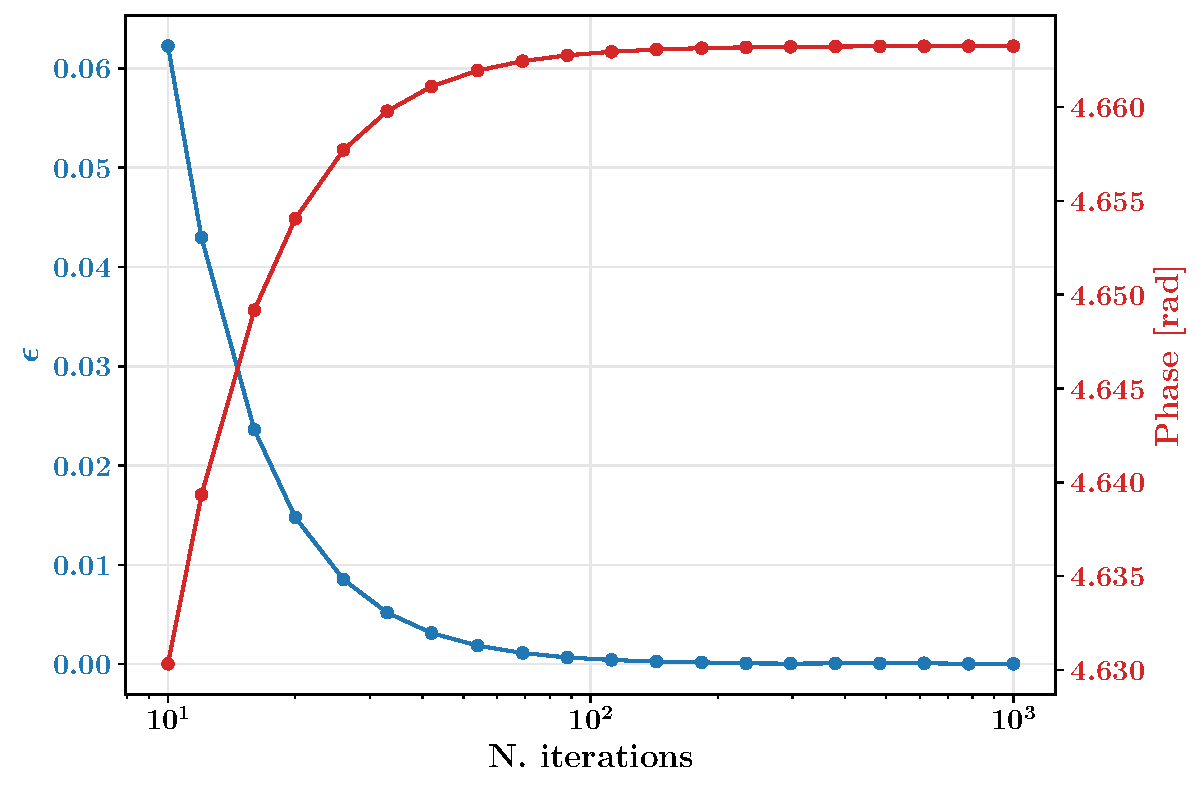
\includegraphics[width=0.7\textwidth]{images/timing/numpy_iter_fidelity_phase.pdf}
    \caption{Phase and error of state $\ket{11}$ as a function of the number of iterations for two-qubits CZ gate. We consider NumPy implementation with Crank-Nicolson with LU decomposition method.}
    \end{figure}
\end{frame}

\begin{frame}[c]{Timing analysis}
\framesubtitle{NumPy}
    \begin{figure}[H]
    \centering
    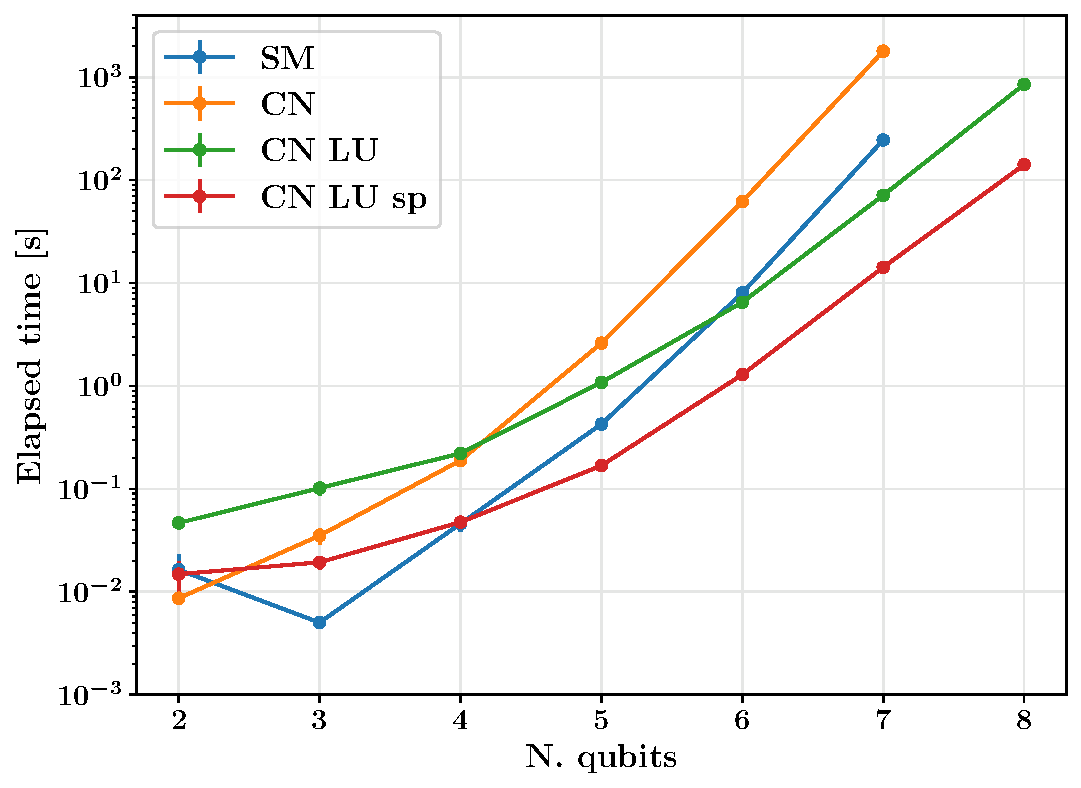
\includegraphics[width=0.7\textwidth]{images/timing/time_numpy.pdf}
    \caption{Mean elapsed time in seconds as a function of the number of qubits in the chain. Spectral Method (SM), Crank-Nicolson method (CN),  Crank-Nicolson with LU decomposition method (CN LU) and Crank-Nicolson with LU decomposition with sparse matrix method (CN LU sp) are compared.}
    \end{figure}
\end{frame}

\begin{frame}[c]{Timing analysis}
\framesubtitle{TensorFlow CPU and GPU}
\begin{figure}[H]
\begin{minipage}[c]{0.49\linewidth}
\subfloat[][TensorFlow CPU]{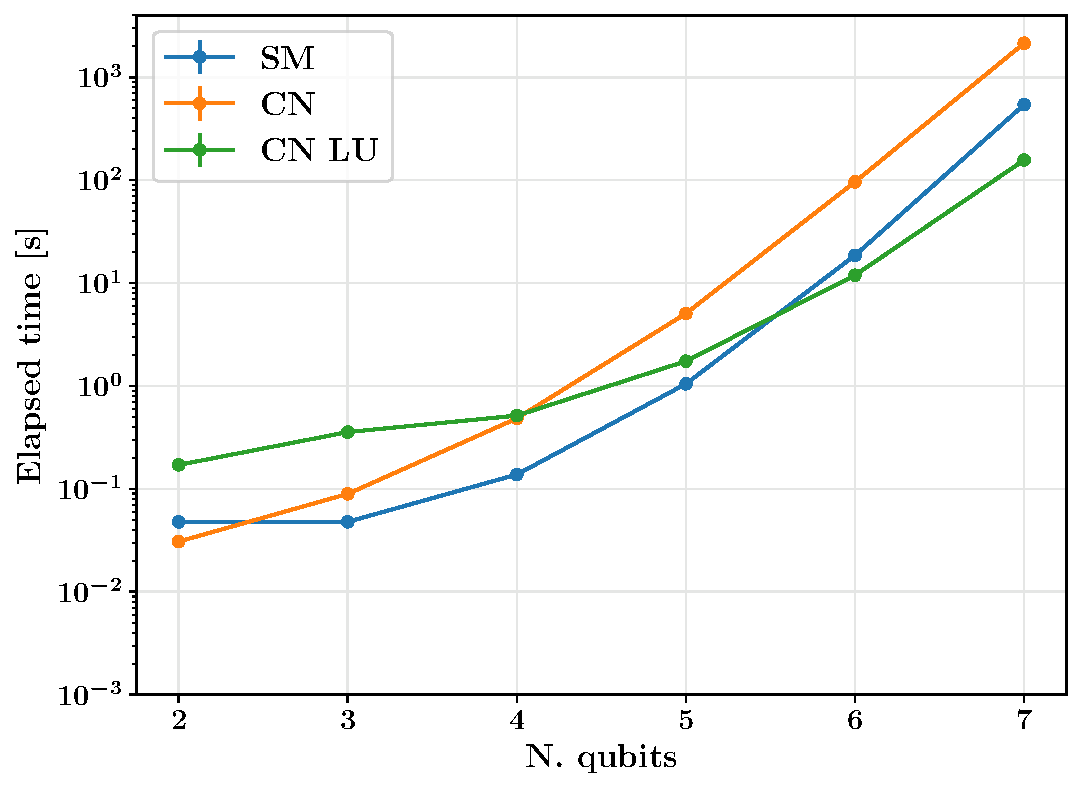
\includegraphics[width=1.0\textwidth]{images/timing/time_tensorflow_CPU.pdf} \label{fig:tensor_CPU} }
\end{minipage}
\begin{minipage}[]{0.49\linewidth}
\centering
\subfloat[][TensorFlow GPU]{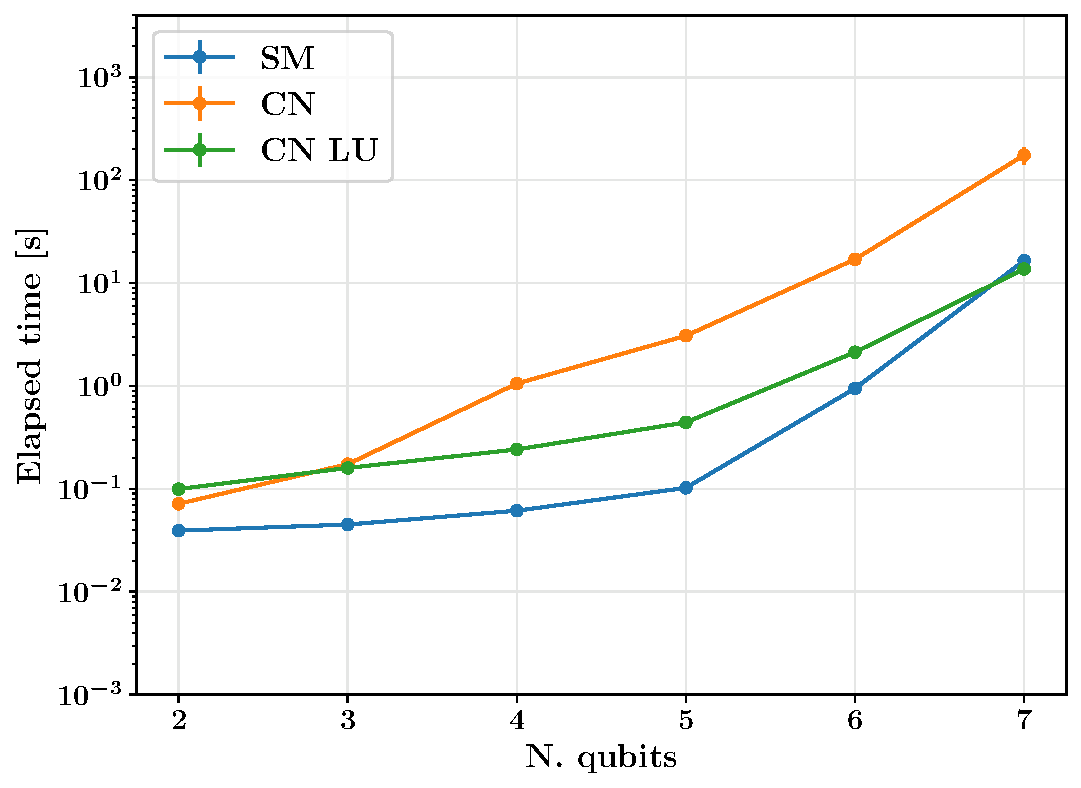
\includegraphics[width=1.0\textwidth]{images/timing/time_tensorflow_GPU.pdf}  \label{fig:tensor_GPU} }
\end{minipage}
\caption{Mean elapsed time in seconds as a function of the number of qubits in the chain. Spectral Method (SM), Crank-Nicolson method (CN) and Crank-Nicolson with LU decomposition method (CN LU) are compared.}
\label{fig:timing}
\end{figure}

\end{frame}

\begin{frame}[c]{Timing analysis}
\framesubtitle{Spectral methods comparison}
    \begin{figure}[H]
    \centering
    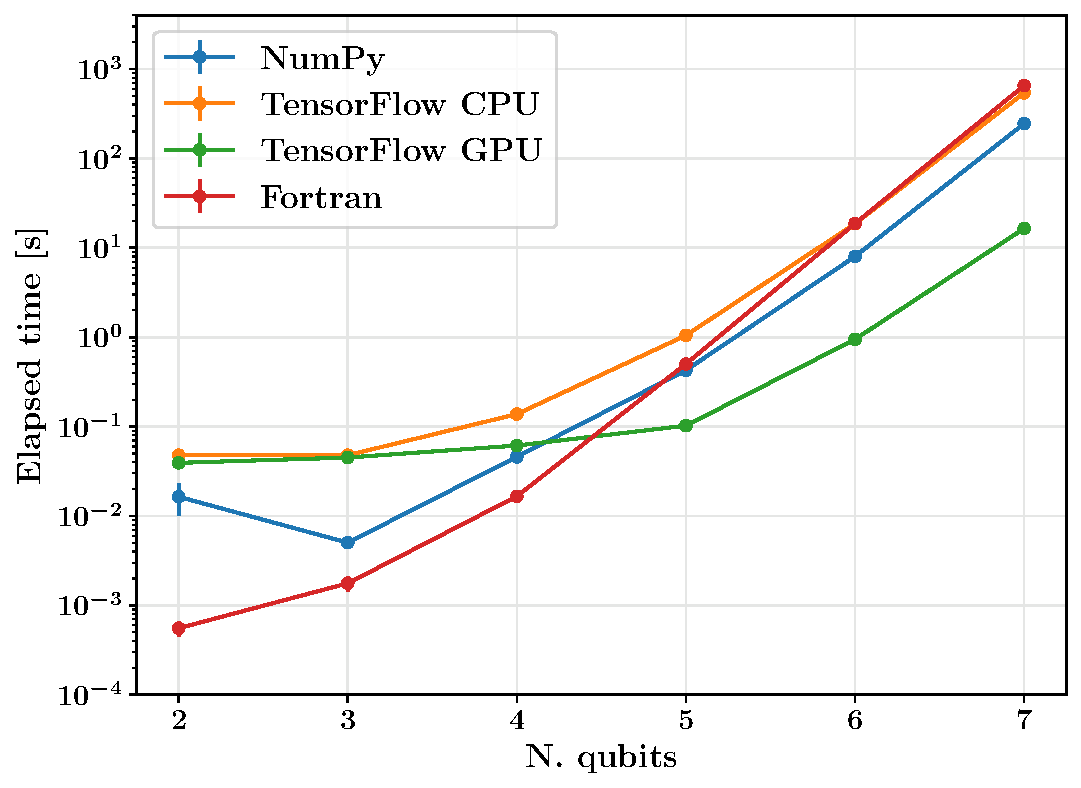
\includegraphics[width=0.7\textwidth]{images/timing/timing_spectral_comparison.pdf}
    \caption{Mean elapsed time in seconds as a function of the number of qubits in the chain.}
    \end{figure}
\end{frame}


\begin{frame}{Conclusions}
\framesubtitle{~}  
\begin{itemize}
    \item \textbf{Gaussian noise} is introduced to perturb separately the parameter $\Omega\tau$ and $\Delta/\Omega$ $\rightarrow$ no significant differences as a function of the standard deviation of the normal noise for different number of qubits.
    \item \textbf{Timing analysis} $\rightarrow$ for a lower number of qubits the Spectral Method have good performances but it is not feasible for large number of qubits. Approximation are needed in order to handle such big matrices $\rightarrow$ Crank-Nicolson
\end{itemize}
\end{frame}	

%%%%%%%%%%%%%%%%%%%%%%%%%%%%%%%%%%%%%%%%%%%%%%%%%%%%%%%
\begin{frame}{~}
\framesubtitle{~}  
\begin{center}
    \begin{minipage}[c]{0.55\textwidth}
        \begin{tcolorbox}[colframe=mydarkblue,colback=myblue,coltext=black]            \begin{center}
        \Huge \textbf{Thank you for the attention!}
        \end{center}
        \end{tcolorbox}
    \end{minipage}
\end{center}
\end{frame}	

 \end{document}